\documentclass[a4paper,11pt]{kth-mag}
\usepackage[T1]{fontenc}
\usepackage{textcomp}
\usepackage{lmodern}
\usepackage[utf8]{inputenc}
\usepackage[swedish,english]{babel}
\usepackage{csquotes}
\usepackage{listings}
\usepackage{enumitem}
\usepackage{courier}
\usepackage{epigraph}
\usepackage{modifications}
\usepackage{algorithm}
\usepackage{pifont}
\usepackage{numberedblock}
\usepackage{forest}
\usepackage{subcaption}
\usepackage{pgfplots}
\usepackage{tabu}
\usepackage{fancyvrb}
\usepackage[section]{minted}
\usepackage{standalone}
\usepackage[backend=biber]{biblatex}
\usepackage{hyperref}

\addbibresource{references.bib}

\title{Evaluating the effect of cardinality estimates on two state-of-the-art
  query optimizer's selection of access method}

\foreigntitle{En utvärdering av kardinalitetsuppskattningens påverkan på två
  state-of-the-art query optimizers val av metod för att hämta data}
\author{Martin Barksten}
\date{January 2016}
\blurb{Master's Thesis at NADA\\Supervisor: John Folkesson\\Examiner: Patric Jensfelt}
% \trita{TRITA xxx yyyy-nn}

\begin{document}
\lstset{basicstyle=\ttfamily,breaklines=true}
\lstset{frame=lines}
\emergencystretch=1em
\pgfplotsset{width=10cm, compat=1.9}
\tabulinesep=1.2mm

\makeatletter
\g@addto@macro\@floatboxreset\centering
\makeatother

\newcommand{\json}[5]{
  \inputminted[breaklines, breakanywhere, fontsize=\footnotesize]{json}{#1}
  \captionof{listing}{The output when testing #2 with query #3, a statistics
    target of $#4$ and #5 repetitions.}
}
\newcommand{\clj}[1]{\mintinline{clojure}{#1}}
\newcommand{\sql}[1]{\mintinline{sql}{#1}}
\newenvironment{indexgraph}{
  \begin{tikzpicture}[scale=0.8]
    \begin{axis}[
      ybar,
      legend style={at={(0.5,-0.15)},
        anchor=north,legend columns=-1},
      symbolic x coords={ct,t,mt,mm,book,cmt,cmm,est,resamb},
      nodes near coords,
      ylabel={\#access methods},
      ytick=\empty,
      xtick=data]
} {
  \legend{MariaDB, PostgreSQL}
\end{axis}
\end{tikzpicture}
}

\newenvironment{indexplot}{
\begin{tikzpicture}[scale=0.8]
  \begin{axis}[
    ylabel={\#relations with varying access methods},
    xlabel={target statistic},
    legend style={at={(0.5,-0.2)},
      anchor=north,legend columns=-1},
    xtick={0,1,2},
    ytick={0, 1,2,3,4,5},
    xticklabels={$1$, $d$, $2d$},
    domain=0:2]
}{
  \legend{PostgreSQL, MariaDB}
\end{axis}
\end{tikzpicture}
}

\frontmatter
\pagestyle{empty}
\removepagenumbers{}
\maketitle
\selectlanguage{english}
\begin{abstract}
    This is a skeleton for KTH theses. More documentation regarding the KTH thesis class file can be found in the package documentation.

Lorem ipsum dolor sit amet, consectetuer adipiscing elit. Mauris
purus. Fusce tempor. Nulla facilisi. Sed at turpis. Phasellus eu
ipsum. Nam porttitor laoreet nulla. Phasellus massa massa, auctor
rutrum, vehicula ut, porttitor a, massa. Pellentesque fringilla. Duis
nibh risus, venenatis ac, tempor sed, vestibulum at, tellus. Class
aptent taciti sociosqu ad litora torquent per conubia nostra, per
inceptos hymenaeos.

\end{abstract}
\clearpage
\begin{foreignabstract}{swedish}
    Detta masterexamensarbete behandlar relationella databaseer och hur stor
påverkan kvaliteten på den uppskattade kardinaliteten har på antalet olika
metoder som används för att hämta data från samma relation. Två databaser
testades --- PostgreSQL och MariaDB --- på ett verkligt dataset för att ge
realistiska resultat. Utvärderingen gjordes med hjälp av ett verktyg
implementerat i Clojure och testerna gjordes på en query, och delvarianter av
den, med varierande stora sample sizes för kardinalitetsuppskattningen.

Resultaten indikerar att MariaDBs query optimizer påverkas lite av
kardinalitetsuppskattningen, för alla testerna valde den samma metod för att
hämta datan. Detta skiljer sig mot PostgreSQLs query optimizer som varierade
mellan att använda sig av index eller göra en full table scan beroende på den
uppskattade kardinaliteten. Slutligen, pekade även resultaten på ett båda
databasernas query optimizers varierade metod för att hämta data beroende på
värdet i predikatet som används för att filtrera bort rader.
\end{foreignabstract}
\clearpage
\tableofcontents*
\clearpage
\listoffigures
\mainmatter*{}
\pagestyle{newchap}

\chapter*{Glossary}\label{chap:glossary}
    The terminology of databases often varies across literature and database
vendors, this section therefore defines the terms used through this thesis. When
it is the case that something commonly goes by other names as well, they will be
included to a great an extent as possible.

\subsection*{Database}
No distinction is made between the database and the Database Management Systems
(DBMS) in this thesis as it is not relevant to separate them. If it is relevant
to distinguish between the two it will be done explicitly.

\subsection*{Data}
The \textit{data} in a database is the values stored in the rows and columns of
the database. This does not include additional information stored in the
database such as indexes.

\subsection*{Dataset}
A \textit{dataset} is all information stored in the database, including both
data and additional information such as indexes, primary and foreign keys etc.

\subsection*{Query optimizer}
The terms query optimizer and optimizer are used interchangeably throughout the
thesis. If an optimizer of some other kind is used this will be made explicit.

\subsection*{Host variable}
A \textit{host variable} is a variable declared in the program in which the SQL
statement is embedded~\cite[p. 151]{chamberlin_1998_complete_acgtdud}. Host
variables are distinguished from normal columns by the fact that they begin with
a colon. An example of a host variable is \sql{:HEIGHT} in
Figure~\ref{fig:sql:hostvar}.

\begin{figure}[ht]
  \begin{minted}[breaklines]{sql}
    SELECT  NAME
    FROM    PERSONS
    WHERE   HEIGHT = :HEIGHT
  \end{minted}
  \caption[A query with a host variable]{A simple query using a host
    variable.}\label{fig:sql:hostvar}
\end{figure}

\subsection*{Predicate}
In order to get the data you need, you must be able to specify what conditions
the data should fulfill to be relevant, this is done by specifying predicates.
To illustrate, consider Figure~\ref{fig:sql:predicate} taken
from~\cite{lahdenmaki_2005_relational_rdidatodossea}.

\begin{figure}[ht]
  \begin{minted}[breaklines]{sql}
    WHERE   SEX = 'M'
    AND
    (WEIGHT = 90
    OR
    HEIGHT > 190)
  \end{minted}
  \caption[The \sql{WHERE} clause of a query containing three predicates and two
  compound predicates]{The \sql{WHERE} clause an SQL query containing three
    predicates and two compound predicates.}\label{fig:sql:predicate}
\end{figure}

The \sql{WHERE} clause in Figure~\ref{fig:sql:predicate} contains three
predicates:
\begin{enumerate}
\item \sql{SEX = 'M'}
\item \sql{WEIGHT = 90}
\item \sql{HEIGHT > 190}
\end{enumerate}

A \textit{compound predicate} is two or more predicates that are tied together
in the form \sql{AND}, \sql{OR} or other similar operators. The \sql{WHERE}
clause in Figure~\ref{fig:sql:predicate} can be considered to have two different
compound predicates:
\begin{enumerate}
\item \sql{WEIGHT = 90 OR HEIGHT > 190}
\item \sql{SEX = 'M' AND (WEIGHT = 90 OR HEIGHT > 190)}
\end{enumerate}

\subsection*{Index slice}
The term \textit{index slice} comes
from~\cite{lahdenmaki_2005_relational_rdidatodossea} and is defined as the
number of index rows that need to be read for a predicate; the thinner the slice
the less amount of index rows that need to be read, and consequently the number
of reads to the table.

The thickness of the index slice will depend on the number of \textit{matching
  columns}, that is the number of columns that exist both in the \sql{WHERE}
clause and the index. To illustrate why consider the query in
Figure~\ref{fig:sql:indexslice}.

\begin{figure}[ht]
  \begin{minted}[breaklines]{sql}
    WHERE   WEIGHT = 90
    AND
    HEIGHT > 190
  \end{minted}
  \caption[The \sql{WHERE} clause of a query with two potential matching
  columns]{The \sql{WHERE} clause of a query with two potential matching
    columns.}\label{fig:sql:indexslice}
\end{figure}

If there exists an index on only \sql{HEIGHT}, no values for \sql{WEIGHT} can be
discarded in the index slice. If an index is added for \sql{WEIGHT}, the
thickness of the index slice will decrease as only values fulfilling both the
\sql{HEIGHT} and \sql{WEIGHT} requirements remain.

\subsection*{Indexable predicate}
A \textit{indexable predicate} is a predicate that can be evaluated when the
index is accessed (allowing a matching index scan)~\cite{2014_summary_sopp,
  2013_ibm_ikcianp}. Revisiting the example from earlier, both of the predicates
in Figure~\ref{fig:sql:indexslice} are examples of indexable predicates.

\subsection*{Matching predicate}
A \textit{matching predicate} is an indexable predicate with the corresponding
necessary indexes~\cite{2013_ibm_ikcianp}. In Figure~\ref{fig:sql:indexslice}
both predicates are indexable and would be matching if there exists an index for
\sql{WEIGHT} and \sql{HEIGHT} respectively.

\subsection*{Non-indexable predicate}
A \textit{difficult predicate} (also sometimes called \textit{nonsearch
  arguments}, \textit{index suppression}, \textit{difficult predicate}) is the
opposite of an indexable predicate, and can as a consequence not define the
index slice~\cite{lahdenmaki_2005_relational_rdidatodossea}. What predicates are
non-indexable varies from database to database, but a typical example of one can
be seen in Figure~\ref{fig:sql:nonindexable}.

\begin{figure}[ht]
  \begin{minted}[breaklines]{sql}
    COL1 NOT BETWEEN :hv1 AND :hv2
  \end{minted}
  \caption[An example of a non-indexable predicate]{A example of a commonly used
    non-indexable predicate.}\label{fig:sql:nonindexable}
\end{figure}

\subsection*{Boolean term predicate}
A \textit{boolean term predicate} (BT predicate) is one that can reject a row
because it does not match the
predicate~\cite{lahdenmaki_2005_relational_rdidatodossea}. Conversely a non-BT
predicate is a predicate that cannot reject a row. Non-BT predicates are
typically the result of using \sql{OR}. To illustrate when a predicate is BT
respectively non-BT consider, assume there is an index \texttt{(A, B)} on
\sql{TABLE} and consider Figure~\ref{fig:sql:btpredicate} and
Figure~\ref{fig:sql:nonbtpredicate}.

\begin{figure}[ht]
  \begin{minted}[breaklines]{sql}
    SELECT  A, B, C
    FROM    ATABLE
    WHERE   A > :A
    AND
    B > :B
  \end{minted}
  \caption[A query containing a BT predicate]{A query with a BT
    predicate.}\label{fig:sql:btpredicate}
\end{figure}

\begin{figure}[ht]
  \begin{minted}[breaklines]{sql}
    SELECT  A, B, C
    FROM    ATABLE
    WHERE   A > :A
    OR
    B > :B
  \end{minted}
  \caption[A query containing no BT predicates]{An query with no BT
    predicates.}\label{fig:sql:nonbtpredicate}
\end{figure}

For the query in Figure~\ref{fig:sql:btpredicate} if the first predicate \sql{A
  > :A} evaluates to false for a row the row can be rejected instantly, making
it a BT predicate. For the query in Figure~\ref{fig:sql:nonbtpredicate} on the
other hand it might be the case that \sql{B > :B} evaluates to true even if
\sql{A > :A} does not, making both predicates non-BT predicates.

\subsection*{Index screening}
A column may be in both the \sql{WHERE} clause and the index, yet be unable to
participate in defining the index slice due to other
reasons~\cite{lahdenmaki_2005_relational_rdidatodossea}. Even if this is the
case the column may still be able to reduce the amount of reads to the table
anyway. A column fulfilling these criteria is a \textit{screening column} as the
presence of it in the index allows not reading from the table. The process of
determining which columns might fulfill this is called \textit{index screening}.

\subsection*{Cardinality}
The \textit{cardinality} is the number of distinct values for a column, or
combination of columns~\cite{lahdenmaki_2005_relational_rdidatodossea}. The
cardinality of the data is usually used when the query optimizer estimates the
cost of different access paths.

\subsection*{Filter factor}
The \textit{filter factor} specifies what proportion of the rows that    satisfy
the conditions in a predicate~\cite{lahdenmaki_2005_relational_rdidatodossea}.
The filter factor can be seen as the selectivity of a predicate and the lower it
is, the more the number of rows that are filtered out by a predicate. For a
predicate such as \sql{HEIGHT = :HEIGHT} there are three ways to talk about
filter factor:
\begin{itemize}
\item The \textit{value specific filter factor} is the filter factor for one
  specific value of \sql{:HEIGHT};
\item The \textit{average filter factor} is the average value for all value
  specific filter factors;
\item And the \textit{worst-case filter factor} is the highest possible filter
  factor for a given value of \sql{:HEIGHT}
\end{itemize}

\subsection*{Access path}
The query optimizers output is an \textit{access path}, which is an abstract
representation of the path to access the data.

\subsection*{Execution plan}
The \textit{execution plan} corresponds to an access path but describes how to
physically access the data.

\subsection*{Query plan}
The \textit{query plan} is the plan suggested by the database for how to access
the data. It is the database-specific description of the access path.


\mainmatter{}
\chapter{Introduction}\label{chap:introduction}
    \epigraph{The person who gave us this book told us that the book describes a
  secret technology called a database.\\
  We hear that the database is a system that allows everyone to share, manage, and
  use data.}{\textit{The King of Kod, from~\cite[p.
    6]{takahashi_2009_manga_tmgtd}}}

If you want to save data, you need a database. And almost every computer program
need to save some form of data, consequently requiring them to use a database.
The trend is also going towards generating more and more data, putting higher
strain on databases and requiring better performance. To improve and develop
databases is therefore a topic of much relevance in today's society.

One key component of databases is the query optimizer, the part of the database
that analyses the users query and finds the optimal path to access it. Or
rather, theoretically it finds the optimal path. Work has been done improving
query optimizers since the early '70s~\cite{chaudhuri_1998_overview_aooqoirs},
yet optimizers often select a bad access path, causing slow
queries~\cite{leis_2015_how_hgaqor}.

Guy Lohman identifies the cardinality estimate of the data to be main cause for bad plans:

\textit{``The root of all evil, the Achilles Heel of query optimization, is the
  estimation of the size of intermediate results, known as cardinalities''}

The estimates can often be wrong by several orders of
magnitude~\cite{lohman_query_iqoap}. These incorrect estimates then propagate
through the query and grow at an exponential
rate~\cite{ioannidis_1991_propagation_otpoeitsojr}, making the query optimizer
base its decisions on false grounds.

The topic of improving the estimations has seen some study, yet the evaluation
of new methods is often done on data that is easy to estimate, being uniformly
distributed. It is only recently that a study has been done to analyze the
performance of the optimizer end-to-end on complex real-world
data~\cite{leis_2015_how_hgaqor}. As one of the results, the study found that
PostgreSQL's optimizer performs unnaturally well on the typically tested uniform
data.

This thesis will aim to provide further insight into performance of
query optimizers by studying a previously unstudied metric and analysing the
performance of state-of-the-art optimizers. The evaluation will be conducted on
complex real-world data.

\section{Problem statement}
In this thesis two open-source state-of-the-art databases are evaluated:
MariaDB~\cite{mariadb_m} and PostgreSQL~\cite{postgresql_ptwmaosd}. One
real-world dataset containing a large amount of data and with a complex schema
and setup will be used in the evaluation. The database will be analyzed to
measure the performance of the query optimizer in order to answer the question:

\textit{How much effect does the cardinality estimate have on the query optimizers
  selection of access method during the join enumeration?}

To evaluate this tests will be done in order to identify a correlation between
the quality of the cost estimation and the number of different access methods
used. To simulate varying, but realistic, quality of the cost estimation the
sample size used to estimate the cardinality will be varied. For a more in-depth
description of how this evaluation is conducted, see Section~\ref{sec:choiceofmethod}.

The exact setup and metrics of the dataset is described in
Section~\ref{sec:benchmark}. A motivation to why the databases are used is
described in Section~\ref{sec:choiceofdatabases}.

\section{Purpose}~\label{sec:purpose}
Query optimizers make bad cardinality estimates, and as a consequence bad cost
estimations of access paths~\cite{leis_2015_how_hgaqor} – but how much does this
affect the actual selection of access method? Even though the errors may be large,
they may not be sufficiently large to actually cause the optimizer to generate
different access paths.

There are three steps to the optimization – search space expansion, cost
estimation and join enumeration (more about those in Section~\ref{sec:queryopt})
– this thesis will focus on measuring what effect bad performance in the first
two steps has on the third and final one. The focus of the study will be to
identify if cost estimation does affect the access methods used and if the
behavior differs between the databases evaluated. Finding an answer to these two
will give a good indication to what effect the cost estimation has on the final
step in terms of access methods used.

Studying this is of relevance for the following reasons:
\begin{enumerate}
\item\label{item:purpose:tool} The tool developed for evaluation can be used
  in the future to measure the performance of query optimizers;
\item\label{item:purpose:steps} The evaluation will provide insight into
  what steps in the optimization process produce bad access paths;
\item\label{item:purpose:data} The performance of query optimizers has not
  seen much study using actual real-world data;
\item\label{item:purpose:performance} The actual performance of the
  databases right now will be evident;
\item\label{item:purpose:compare} Since both databases compared are
  open-source, one performing better may guide development for the other.
\end{enumerate}

Of primary interest for academia are probably
reasons~\ref{item:purpose:tool},~\ref{item:purpose:steps}
and~\ref{item:purpose:data} whereas database vendors might be more interested
in~\ref{item:purpose:performance} and~\ref{item:purpose:compare}.

\section{Outline}
Below is a brief outline of the chapters in the report and what can be expected
to be found in each:

\begin{itemize}
\item The \nameref{chap:introduction} chapter gives an introduction to the
  subject, the problem statement discussed, the purpose of
  the thesis and why it is novel and relevant.
\item The \nameref{chap:relatedwork} chapter contains an overview of what
  previous and relevant work has been done in the area of improving and
  evaluating the performance of query optimizers.
\item The \nameref{chap:theory} chapter gives a background and the information
  necessary to understand the thesis. The chapter begins with a background on
  how a modern query optimizer works. It then continues with a description of
  the individual characteristics of the databases analysed: MariaDB and
  PostgreSQL.\@ It also defines some important terms used throughout the thesis.
\item The \nameref{chap:method} chapter describes the evaluations done and how they
  were implemented. It also describes more in-detail the data used for the
  databases, the database configurations used and the environment the tests were
  run in.
\item The \nameref{chap:results} chapter displays the results from the
  performance test in the form of graphs. It also gives some brief commentary on
  them.
\item The \nameref{chap:discussion} chapter discusses the performance of the
  query optimizers and the consequences of it, as well as the validity of the
  results. It also answers the problem statement and provides suggestions for
  future research.
\end{itemize}
\chapter{Related work}\label{chap:relatedwork}
    Improving the query optimizer is a topic naturally tied to that of evaluating
the query optimizer's performance. In spite of this, the optimizer's performance
has not seen much study, while improving them on the other hand has. This
section will start with a section about some of the more recent evaluations that
have been done and then continue with a section about some improvements done to
the query optimizer relating cardinality estimation. A final section describes
some implementations to improve the performance of relational operators and make
them more resistant to bad plans.

\section{Evaluating the query optimizer's performance}
In~\cite{leis_2015_how_hgaqor} Leis et.\ al.\ perform what they claim is:

\textit{``the first end-to-end study of the join ordering problem using a
  real-world data set and realistic queries''}.

In the study they create the a database setup based on the Internet Movie
Database (IMDb), create a set of realistic queries for it and call it the Join
Order Benchmark (JOB). Using this benchmark they then measure how PostgreSQL,
HyPer and three unnamed commercial databases perform in terms of cardinality
estimates, cost modelling and general performance. They also compare the results
to TPC-H, the database setup previously mostly used for evaluation and show that
the PostgreSQL optimizer performs unrealistically well for TPC-H because of the
uniform data distribution. The results of their study show that relational
databases produce large estimation errors and that primarily the cardinality
estimate is to blame.

Another article that has evaluated optimizers
is~\cite{wu_2013_predicting_pqetaocmru} where Wu  et\ al.\ analyzed if the
optimizer's cost model can be used to estimate the actual run-time of the query.
They find that the optimizer consistently makes bad cost estimates, but show
that for analyzing actual run-time a more costly and precise analysis can be
conducted on the selected access path.

Evaluating a query optimizer's cardinality estimation is often done through a
comparison with the actual cardinality. Calculating the exact cardinality can
however be very costly for complex queries and datasets. A more efficient method
that can find the exact cardinalities by studying a subset of all expressions is
presented in~\cite{chaudhuri_2009_exact_ecqofot}.

One novel way of studying and analyzing the plans chosen by the query optimizer
is a tool called Picasso, which allows query plans to be visualized as
two-dimensional diagrams~\cite{haritsa_2010_picasso_tpdqov}. The tool provides a
visualisation of the performance across the entire query plan space, thus
providing another way of analysing queries or query optimizers.

An example of a visualisation done with Picasso can be seen in
Figure~\ref{fig:picasso}. The colored regions represent a specific execution
plan, the X and Y-axis represent the selectivity for the attributes
\sql{SUPPLIER.S_ACCTBAL} and \sql{LINEITEM.L_EXTENDEDPRICE} respectively. The
percentages in the legend correspond to the area covered by each plan.

\begin{figure}[ht]
  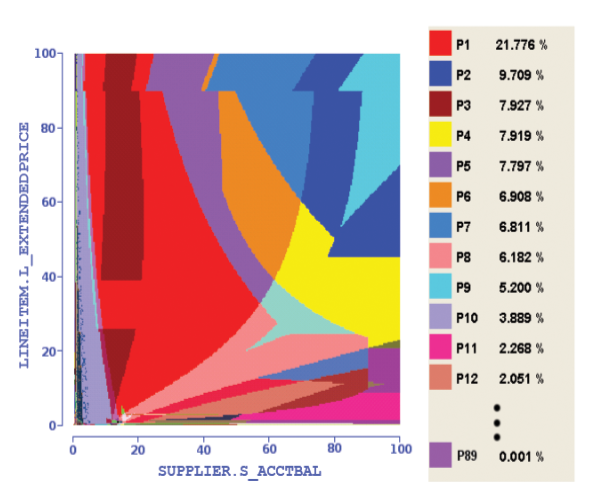
\includegraphics[scale=0.6]{Images/Picasso.png}
  \caption[A query plan visualisation done by Picasso]{A query plan
    visualisation done by Picasso, image taken
    from~\cite{haritsa_2010_picasso_tpdqov}.}\label{fig:picasso}
\end{figure}

Finally, on a more practical note Lahdenmäki  et\ al.\ describe of how to
identify queries where the selected access path is bad, and how to solve the
problem~\cite{lahdenmaki_2005_relational_rdidatodossea}. The book gives a
thorough introduction to many important aspects of the database and the chapter
``Optimizers Are Not Perfect'' focuses on incorrect cardinality estimates and
other common query optimizer errors.

\section{Bad statistics and cardinality estimates}
In~\cite{ioannidis_1991_propagation_otpoeitsojr} Ionnidis  et\ al.\ develop a
framework to study how cardinality estimate errors propagate in queries. Their
results indicate that the error increases exponentially with the number joins.

There are two different methods of improving how optimizers handle cardinality
estimation:
\begin{itemize}
\item Reducing the effect of incorrect estimations by making plans more
  \textit{robust}, which means they perform better over large regions of the
  search space;
\item Or by improving the estimations.
\end{itemize}

\subsection{Improving robustness}
Harish et\ al.\ present a way to make plans more robust by allowing the
optimizer to select the most robust plan that is not ``too slow'' compared to
the calculated optimal path.~\cite{harish_2008_identifying_irptpdr}. They
develop an external tool for this purpose and find that the tool indeed does
improve performance by reducing the effect of selectivity errors.

A similar study is done by Abhirama et\ al.\ but they implement the selection
directly in the PostgreSQL query
optimizer~\cite{abhirama_2010_stability_otsopcatcops}. Their results agree with
those found by Harish  et\ al.\ in that the performance is improved. The results
they present show that robut plans often reduced the adverse effects of
selectivity errors by more than two-thirds, while only providing a minor overhead in
terms of time and memory.

\subsection{Improving cardinality estimates}\label{sec:improving_cardinality_estimates}
The most studied problem of cardinality estimate is that of finding the right
balance between calculation time, memory overhead and correctness. One common
method used in current state-of-the-art databases is histograms that assume
attributes are independent of each other, an assumption that often is not
correct~\cite{ioannidis_2003_history_thoha}. Recent studies have been done to
find alternatives method that do not assume independence.

Tzoumas et\ al.\ present one method that instead of the usual one-dimensional
statistical summary, saves it as a small, two-dimensional
distribution~\cite{tzoumas_2011_lightweight_lgmfsewia}. Their results show an
small overhead, and an order of magnitude better selectivity estimates.

In~\cite{yu_2013_cs2_candsfqea} Yu et\ al.\ develop a  method called
\textit{Correlated Sampling} that does not sample randomly, but rather save
correlated sample tuples that retain join relationships. They further develop an
estimator, called reverse estimator, that use correlated sample tuples for query
estimation. Their results indicate that the estimator is fast to construct and
provides better estimations than existing methods.

In~\cite{vengerov_2015_join_jsestfc} Vengerov et\ al.\ once again study
Correlated Sampling, but improve on it by allowing it to only make a single pass
over the data. They compare the algorithm to two other sampling approaches
(independent Bernoulli Sampling and End-Biased Sampling, which is described
in~\cite{estan_2006_end_esfjce}) and find Correlated Sampling to give the best
estimates in a large range of situations.

\section{Improving operators}
In~\cite{muller_2015_cache_cahis} Müller  et\ al.\ study the two implementations
of relational operators: hashing and sorting (more about these in
Section~\ref{sec:opimpl}). Their study find that the two paradigms are in terms
of cache efficiency actually the same and from this observation develop a
relational aggregation algorithm that outperform state-of-the-art methods by up
to 3.7 times.

A problem described in~\cite{leis_2015_how_hgaqor} is that the optimizer tends
to pick nested-loop joins (more about these in Section~\ref{sec:nestedloopjoin})
even though they provide a high risk but only a very small payoff.
In~\cite{graefe_2011_generalized_agja} Goetz Graefe provides a generalized join
algorithm that can replace both merge joins and hash joins in databases, thus
avoiding the danger of mistaken join algorithm choices during query
optimization.

\chapter{Theory}\label{chap:theory}
    \epigraph{An SQL query walks into a bar and sees two tables.\\
  He walks up to them and asks ``Can I join you?''}{\textit{– Source: Unknown,
    from~\cite{join_tjo}}}

In this chapter a background is given to relational databases with more focus on
the areas of interest for this thesis. The first section will give a high-level
introduction to relational databases and how they work in general. Following
this is a section with a more in-depth description of indexes. After this comes
the final section covering the query optimizer, detailing how it works, how it
can be monitored and its limitations.

\section{Relational databases}
A database is a computerized record-keeping system, a way to save computerized
data~\cite[p. 6]{date_2003_introduction_aitds}. The data stored in the database
can then be accessed and modified by the user. Accessing and modifying the data
is typically done through a layer of software called the database management
system, which provides a method for accessing and modifying the data.

A database stores data in the form of rows in different tables. These rows are
also sometimes referred to as tuples. In a relational database these tuples can
then have relations between each other in the form of for example ``Tuple A has
one or more of Tuple B''.

The following sections will describe some components of the database which are
of the most relevant for this thesis.  First comes a section describing the most
common method to access data in a relational database, SQL, after this is is a
section about how the query described by SQL is executed and finally a section
about one of the most fundamental operations in SQL – the join operation.

\subsection{SQL}
SQL, or Structured Query Language in full, is the computer language most
commonly used to query and modify the database, it is formally defined by
ISO/IEC 9075~\cite[p.
29]{garcia-molina_2002_database_dstcb}\cite{iso_i9itdlsp1f}. The language came
from research into manipulating databases in the early '70s and it is now one of
the most popular database languages in existence~\cite{sql_s|cl}.

\subsection{Query execution}
The execution of a query in the form of an SQL statement is split into four
phases~\cite{selinger_1979_access_apsiardms}:
\begin{enumerate}
\item \textit{Parsing}, in which the input text is transformed into query
  blocks;
\item \textit{Optimization}, in which an optimized way to access the data is
  found, called an \textit{access path};
\item \textit{Code generation}, in which the access path is transformed a way to
  execute it, an \textit{execution plan};
\item And \textit{execution}, when the code is executed;
\end{enumerate}

The \textit{parsing}, \textit{code generation} and \textit{execution phases} are
all fairly trivial compared to the \textit{optimization}. The optimization
process is also the phase that has the potentially most effect on the execution
time for the query. The query optimization process is performed by the query
optimizer, which is described in more detail in Section~\ref{sec:queryopt}.

\subsection{The join operation}
One of the most fundamental operations in SQL is that of joining two tables. An
example of an inner join on the tables \sql{EMPLOYEES} and \sql{DEPARTMENTS} can
be found in Figure~\ref{fig:sql:joinop}.

\begin{figure}[ht]
  \begin{minted}[breaklines]{sql}
    SELECT *
    FROM   EMPLOYEES, DEPARTMENTS
    WHERE  EMPLOYEES.DEPARTMENT_ID = DEPARTMENTS.DEPARTMENT_ID
    AND    EMPLOYEES.NAME = 'John';
  \end{minted}
  \caption[An example of an SQL query]{An SQL query that will find the all
    employees by the name of John and info about their
    department.}\label{fig:sql:joinop}
\end{figure}

There are four kinds of joins typically supported in databases. To illustrate
this assume we have the following \texttt{Join(A, B)}, where \texttt{A} and
\texttt{B} are tables and \texttt{Join} is one of the join operations.
\begin{itemize}
\item An inner join will return all rows in common between \texttt{A} and
  \texttt{B};
\item A left outer join will return all rows in \texttt{A} and all common rows
  in \texttt{B};
\item A right outer join will return all rows in \texttt{B} and all common rows
  in \texttt{A};
\item And a full outer join will return all rows in \texttt{A} and all rows in
  \texttt{B}.
\end{itemize}
See Figure~\ref{fig:vennjoin} for a visualization of the joins using Venn
diagrams.

\begin{figure}[ht]
  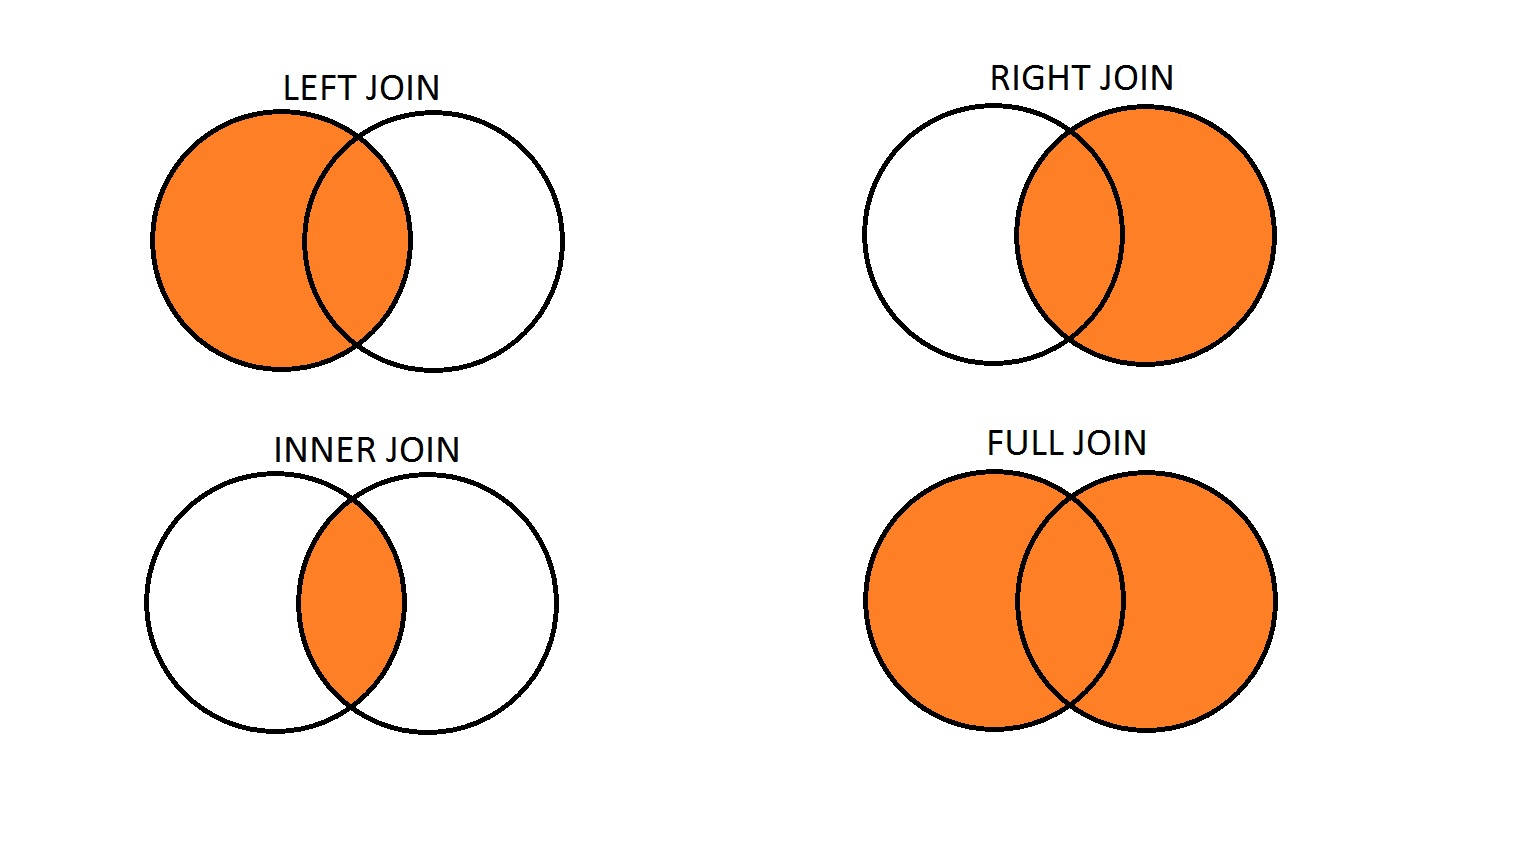
\includegraphics[scale=0.4]{Images/SQL-Join-Venn-Diagrams.jpg}
  \caption[Illustration of join operations using Venn diagrams]{The four join
    operations illustrated using Venn diagrams, image taken
    from~\cite{brian_2014_better_bqj}.}\label{fig:vennjoin}
\end{figure}

\subsection{Implementation of operators}\label{sec:opimpl}

Operators can be divided into three classes:
\begin{enumerate}
\item\label{item:classop:sort} \textit{Sorting-based} methods;
\item\label{item:classop:hash} \textit{Hash-based} methods;
\item\label{item:classop:index} And \textit{index-based} methods.
\end{enumerate}
In general index-based methods are variations of class~\ref{item:classop:sort}
or~\ref{item:classop:hash} that utilize indexes to speed up parts of the
algorithm. Most notably when there exists an index, for example B-trees, that
allows the data to be accessed sorted joins can be done very efficiently.

Furthermore the algorithms for the operators can be divided by the number of
passes the algorithm does:
\begin{enumerate}
\item \textit{One-pass algorithms} read the data from disk only once;
\item \textit{Two-pass algorithms} reads the data once, processes it and saves
  it in some way before doing another pass;
\item And algorithms that do three or more passes, which are essentially
  generalizations of two-pass algorithms.
\end{enumerate}

There are several operators to implement in a database, but the most relevant
algorithms for this thesis are those implementing the join operator.
Implementation of the join operator is typically done with three fundamental
algorithms: nested loop join, merge join and hash join~\cite{postgresql_pd9p}.
Many databases support more join algorithms, but they are typically variations
of one of these three algorithms.

For the descriptions of the algorithms assume we have a query joining the tables
\texttt{A} and \texttt{B}, \texttt{Join(A, B)}. The first table of the join
operation, \texttt{A}, is referred to as the \textit{outer table} and the second
table, \texttt{B}, as the \textit{inner table}.

\subsubsection{Nested loop join}\label{sec:nestedloopjoin}
A nested loop join is essentially two nested loops, one over the outer table and
inside it one over the inner table~\cite[p.
718-722]{garcia-molina_2002_database_dstcb}. The nested loop join is a bit of a
special case as it is not necessarily of any of the classes. The number of
passes it does can also be considered to be ``one-and-a-half'' as the outer
table's tuples is read only once, while the inner table's tuples are read
repeatedly.

If an index exists for the inner table the nested loop join could be considered
to be of class~\ref{item:classop:index} and is then called a \textit{index
  nested loop join}.

\subsubsection{Merge join}
A merge join (sometimes also called \textit{sort-merge join}) is a variation of
a nested loop join that requires both tables to be sorted. The two tables can
then be scanned in parallel, allowing each row to only be scanned
once~\cite[p. 723-730]{garcia-molina_2002_database_dstcb}. The sorting of the
tables can be achieved through an explicit sort step or through an index.

A merge join can be considered to be a two-pass algorithm of
class~\ref{item:classop:sort}.

\subsubsection{Hash join}
There are several types of hash joins but the general principle remains the
same: build a hash table for the outer table, then scan the inner table to find
rows that match the join condition~\cite[p.
732-738]{garcia-molina_2002_database_dstcb}.

Hash joins are two-pass algorithms of class~\ref{item:classop:hash}.

\section{Indexes}
This section will cover the basics behind indexes as described by Ramakrishnan
et.\ al.\ in~\cite[Ch. 8]{ramakrishnan_2003_database_dms}.

An index is a data structure that allows data stored in the database to be
accessed quicker through some retrieval operations. The data stored in the index
is called the \textit{data entry} and the value that is indexed – the value in
the column – is called the \textit{search key}. There are three alternatives for
what to store as the data in the data entry:

\begin{enumerate}
\item\label{item:indexes:alt1} A data entry is a the actual data saved;
\item\label{item:indexes:alt2} A data entry is a pair containing a search key
  and record id;
\item\label{item:indexes:alt3} A data entry is a pair containing a search key
  and a list of record ids corresponding to the key.
\end{enumerate}

Which alternative is used depends on how the index is created and what kind of
an index it is.

\subsection{Composite indexes}
Composite indexes are indexes containing more than one fields. A composite index
can support a broader range of queries than a normal index and since they also
contain more columns, they contain more information about the data saved.

\subsection{Clustered index}
A clustered index is an index on a column which is sorted in the same way as the
index; otherwise it is an unclustered index. An index using
Alternative~\ref{item:indexes:alt1} is sorted by definition, whereas
Alternative~\ref{item:indexes:alt2} and~\ref{item:indexes:alt3} require the data
stored to be sorted.

\subsection{Data structures}
The two most common indexes used are \textit{hash-based indexes} and
\textit{tree-based indexes}. Below is a more detailed description of both.

\subsubsection{Hash-based indexes}
A hash-based index is implemented as a hash table, mapping the hashed value of a
search key to a bucket containing one or more values. To search in the index the
search key is hashed and the corresponding bucket is identified, all values in
the bucket are then examined to identify the matching one.

\subsubsection{Tree-based indexes}
Tree-based indexes save the data as hierarchical sorted trees where the leaf
nodes contain the values. To find a value the search starts at the root and all
non-leaf nodes direct the search toward the correct leaf node. In practice the
trees are often implemented as $B^{+}$-trees, which is a data structure that
ensure that paths from the root to a leaf node are of the same
length~\cite{comer_1979_ubiquitous_ub}. The efficiency of a B-tree index depends
on the number of levels the B-tree has~\cite[p.
645]{garcia-molina_2002_database_dstcb}.

\section{The query optimizer}\label{sec:queryopt}
In order to access the data in an as efficient way as possible, the query is
optimized by a built-in tool in the databases called the query optimizer. Below
is a description of the fundamental operations performed by query optimizer,
taken mostly from C., Surajits article on the
topic~\cite{chaudhuri_1998_overview_aooqoirs}.

Query evaluation is handled by two components: the \textit{query optimizer} and
the \textit{query execution engine}. The input to the query optimizer is a
parsed representation of the SQL query and the output is an execution plan that
the query execution engine then performs.

In order for the query optimizer to find an access path it must be able to:
\begin{enumerate}
\item Expand the \textit{search space} to find all access paths that are valid
  transformations of the query;
\item Perform a \textit{cost estimation} for each access path to calculate its
  cost;
\item And finally \textit{enumerate} the access paths to find which is the best.
\end{enumerate}

A good query optimizer is one that does not cause too much overhead in the query
execution in calculating the access path, while still finding a good access
path. In order to do this each step must fulfill the criteria:
\begin{enumerate}
\item The search space includes plans with a low cost;
\item The cost estimation is accurate;
\item And the enumeration algorithm is efficient.
\end{enumerate}

\subsection{Expanding the search space}
The first task of the query optimizer is that of taking the original search
space containing just the original query, and expanding it through
transformation rules. The expansion will thus generate a larger search space
containing valid permutations of the join order. The output is a set of
\textit{operator trees}, which are binary trees where nodes represent operations
and leaves values.

There are multiple rules that can be applied, most of which are complex and work
only under some specific conditions. The most relevant rules for index-selection
are described below, for a more in-depth description
see~\cite{chaudhuri_1998_overview_aooqoirs}.

\subsubsection{Join reordering}
One important rule is that both inner join and full join are:
\begin{itemize}
\item commutative: \texttt{Join(R1, R2)} is equivalent to \texttt{Join(R2, R1)};
\item Associative, \texttt{Join(R1, Join(R2, R3))} is equivalent to
  \texttt{Join(Join(R1, R2), R3)}.
\end{itemize}
This means that the joins can be grouped and reordered as the optimizer finds
best. Another consequence of this is that the operators that can be seen as a
single node with many children, see Figure~\ref{fig:groupop} for an example.

\begin{figure}[ht]
  \begin{subfigure}[b]{0.5\linewidth}
    \centering
    \begin{forest}
      [\texttt{JOIN}
      [\texttt{JOIN}
      [\texttt{JOIN}
      [\texttt{R}]
      [\texttt{JOIN}
      [\texttt{S}]
      [\texttt{T}]]]
      [\texttt{U}]]
      [\texttt{JOIN}
      [\texttt{V}]
      [\texttt{W}]]]
    \end{forest}
    \caption{\label{fig:groupop:a}}
  \end{subfigure}
  \begin{subfigure}[b]{0.5\linewidth}
    \centering
    \begin{forest}
      [\texttt{JOIN}
      [\texttt{JOIN}
      [\texttt{R}]
      [\texttt{S}]
      [\texttt{T}]]
      [\texttt{U}]
      [\texttt{V}]
      [\texttt{W}]]
    \end{forest}
    \caption{\label{fig:groupop:b}}
  \end{subfigure}
  \caption[An example of how operators can be grouped into a single node]{The
    \texttt{JOIN} operators are assumed to be associative and commutative,
    allowing Figure~\ref{fig:groupop:a} to be transformed into
    Figure~\ref{fig:groupop:b}, example taken from~\cite[p.
    791]{garcia-molina_2002_database_dstcb}.}\label{fig:groupop}
\end{figure}

\subsubsection{Pushing operations up and down the tree}
Another fundamental rule used by optimizers is that of pushing an operator down
the expression tree in order to reduce the cost of performing it~\cite[p.
768-792]{garcia-molina_2002_database_dstcb}. For the example the selection
operators tend to reduce the size of the relations, meaning pushing them down as
far down the tree as possible is beneficial.

Another rule that can be applied is to pull an operator up the tree, in order to
then be able to push it down again to reduce the size of more relations. See
Figure~\ref{fig:pushop}, which illustrate how pulling a selection up the tree
allows it to then be pushed down more branches.

The conditions for when these rules are applicable naturally varies a lot
depending on the operator and it is beyond the scope of this thesis to list them
all. See~\cite[p. 768-779]{garcia-molina_2002_database_dstcb} for an in-depth
description of the rules and conditions.

\begin{figure}[ht]
  \begin{subfigure}[b]{0.5\linewidth}
    \centering
    \begin{forest}
      [\texttt{starName, studioName}
      [\texttt{JOIN}
      [\texttt{year = 1996}
      [\texttt{Movies}]]
      [\texttt{StarsIn}]]]
    \end{forest}
    \caption{\label{fig:pushop:a}}
  \end{subfigure}
  \begin{subfigure}[b]{0.5\linewidth}
    \centering
    \begin{forest}
      [\texttt{starName, studioName}
      [\texttt{JOIN}
      [\texttt{year = 1996}
      [\texttt{Movies}]]
      [\texttt{year = 1996}
      [\texttt{StarsIn}]]]]
    \end{forest}
    \caption{\label{fig:pushop:b}}
  \end{subfigure}
  \caption[Illustrating how operators can be pushed and pulled up and down the
  tree]{An expression tree representing a query to find which stars worked for
    which studios in 1996, example taken~\cite[p.
    774]{garcia-molina_2002_database_dstcb}. The selection operator in
    Figure~\ref{fig:pushop:a} is first pulled up the tree, allowing it to then
    be pushed down an additional branch as illustrated in
    Figure~\ref{fig:pushop:b}.}\label{fig:pushop}
\end{figure}

\subsubsection{Eliminating operators via an index}
Several operations such as \sql{GROUP BY}, \sql{ORDER BY}, \sql{MAX} etc can be
eliminated because the the relation is known to already fulfill these
criteria~\cite[p. 777-779]{garcia-molina_2002_database_dstcb}. One of the more
common criteria is than index that allows the data to be retrieved sorted
exists.

In combination with the ability to move operators up and down the tree this can
be very powerful as potentially costly operations can be eliminated.

\subsubsection{Accessing table data}
For each read from a table there will be generated one access path per usable
index, as well as one for a full table scan~\cite[p.
827-829]{garcia-molina_2002_database_dstcb}.

\subsection{Cost estimation}
The second task of the query optimizer is to be able to assign a cost to a given
search plan. This cost estimation will be repeated several times as it is called
for each operator tree in the search space that the query optimizer considers
relevant, thus it is important that the estimation is efficient. The cost
estimation is done in three steps:
\begin{enumerate}
\item Collect statistics of stored data;
\item For each node in the tree calculate the cost of applying the operation;
\item And then the calculate the statistics for the resulting output.
\end{enumerate}

There are two important statistics that need to be calculated for the data: the
number of tuples in a relation and the number of different values in the column
of a relation for an attribute~\cite[p.
807-808]{garcia-molina_2002_database_dstcb}. Common methods of saving the data
is through a histogram describing the data distribution for an attribute. If
histograms are not used the second highest and lowest values are used – this is
because the highest and lowest values often are outliers

Modern databases can contain huge amounts of data and thus calculating the exact
histograms is impossible, requiring them to be estimated, usually through
\textit{sampling}~\cite[p. 807-808]{garcia-molina_2002_database_dstcb}. When
estimating via sampling only a subset of the data is read and used to estimate.
Furthermore the statistics are usually only computed periodically as they:
\begin{itemize}
\item Tend not to change radically in a short time;
\item Even if inaccurate, they are used consistently for all cost estimations;
\item And keeping them up to date may cause their calculations to take up the
  most of the database's time.
\end{itemize}

Finally the statistics need to be propagated upwards in the tree. There are
several ways of performing this propagation and they are described in more
detail in~\cite{chaudhuri_1998_overview_aooqoirs}.

\subsection{Enumeration}
The enumeration is the final task of the optimizer and the one that will perform
the actual expansion and cost estimation, as it selects in what way to expand
the search space. It would be too costly to expand the entire search space and
for each plan estimate the cost, instead the search space is expanded
heuristically in a way that the optimizer believes will give cheap plans.

When expanding the search space the general principle is to find paths where the
size of relations is reduced as early as possible. For example pushing an
operation down the tree, as shown in Figure~\ref{fig:pushop}, can reduce the
size of the relation and thus reduce the cost of performing a join later
on~\cite[p. 772-774]{garcia-molina_2002_database_dstcb}.

If the enumeration algorithm estimates the cost for a new plan to be more
expensive than a previously found one, it can discard it right away. The main
goal for the enumeration algorithm is therefore to expand the search space in
such a way that the best plans are generated early, so that the more expensive
plans can be discarded quickly later on~\cite{nica_2012_analyzing_aqoppojea}.

Most modern query optimizers use a dynamic programming algorithm first proposed
in 1979 for the System R database~\cite{selinger_1979_access_apsiardms}. The
algorithm is built on the observation that the join methods are independent,
that is the best join method for joining the composite to relation $i$ is
independent of joining of the first $i-1$ relations. The method used is then to
construct a tree with all permutations of joins by searching from smaller to
successively larger subsets.

One final optimization done during this step is also to heuristically prune
subtrees that the heuristic consider too bad to even
consider~\cite{ono_1990_measuring_mtcojeiqo}.

\subsection{Monitoring}
It is often useful to monitor and see what decisions the query optimizer make
and why; most databases implement the ability to do so via an SQL
statement~\cite[p. 34]{lahdenmaki_2005_relational_rdidatodossea}. In PostgreSQL
and MariaDB the statement is called
\sql{EXPLAIN}~\cite{postgresql_pd9e}~\cite{explain_emkb}, but it is also called
\sql{SHOW PLAN} or \sql{EXPLAIN PLAN}. For an example of how \sql{EXPLAIN} is
used see Figure~\ref{fig:sql:explainquery}, which shows the code for a query,
and Figure~\ref{fig:sql:explaintrace}, which shows the corresponding trace.

\begin{figure}[ht]
  \begin{minted}[breaklines]{sql}
    EXPLAIN
    SELECT  title.title
    FROM    movie_info, title
    WHERE   movie_info.info IN ('Bulgaria') AND movie_info.movie_id=title.id;
  \end{minted}
  \caption[An example query to \sql{EXPLAIN}]{An example of a query done on the
    IMDb dataset, requesting the title of all movies filmed in Bulgaria. See
    Figure~\ref{fig:sql:explaintrace} for the
    output.}\label{fig:sql:explainquery}
\end{figure}

\begin{figure}[ht]
  \begin{lstlisting}
    Merge Join  (cost=2.25..921735.28 rows=19682252 width=17)
    Merge Cond: (title.id = movie_info.movie_id)
    ->  Index Scan using title_pkey on title  (cost=0.43..155884.96 rows=3572150
    width=21)
    ->  Index Only Scan using movie_info_idx_mid on movie_info
    (cost=0.44..511110.22 rows=19682252 width=4)
    (4 rows)
  \end{lstlisting}
  \caption[An example of an \sql{EXPLAIN} trace]{The access path as shown by
    PostgreSQL's EXPLAIN statement, corresponding to the the query in
    Figure~\ref{fig:sql:explainquery}.}\label{fig:sql:explaintrace}
\end{figure}

\subsection{Limitations}
Even though much work has been done on improving query optimizers they may not
always choose the correct access path. This section will describe some of the
primary reasons why an incorrect access path path is chosen, as described
in~\cite[Ch. 14]{lahdenmaki_2005_relational_rdidatodossea}.

\subsubsection{The optimizer can't see the best path}
One reason the query optimizer cannot find the best path is because it is unable
to see all alternatives because the query is too complicated for it.

\begin{itemize}
\item If a predicate is non-indexable it cannot by definition participate in
  defining the index slice. Furthermore it might also be the case when the
  predicate is even more difficult that the the optimizer is unable to perform
  an index screening, forcing it to read a table row.
\item If a compound predicate contains \sql{OR} it may become non-BT, which in
  turn mean the predicate cannot be used to define the index slice. This means
  the query optimizer cannot make full use of potential indexes that exist.
\item Sometimes the optimizer will add an \sql{ORDER BY} to data that is already
  sorted thanks to an index.
\end{itemize}

\subsubsection{The optimizer's cost estimate is wrong}
Even if the optimizer is able to see all alternatives it might be the case that
the filter factor is incorrectly estimated, resulting in an incorrect access
path.

\begin{itemize}
\item If the filter factor is not estimated for a host variable, it must use a
  default value which often results in a poor estimate. However, if the filter
  facotr is estimated evewry time the query is executed it adds a large
  overhead.
\item If the optimizer is unaware of the true distribution of the data it might
  make a guess based on the cardinality, if the distribution is skewed this
  guess may very well become very incorrect.
\item In a compound predicate such as \sql{HEIGHT = :HEIGHT AND WEIGHT =
    :WEIGHT} the optimizer can only produce a good estimate of the filter factor
  only if it knows the cardinality of the combination of the \sql{HEIGHT} and
  \sql{WEIGHT} columns. If it does not, it must somehow estimate this.
\end{itemize}

\chapter{Method}\label{chap:method}
    In this chapter, the method used to investigate the problem statement is
presented. First, the choice of method is described, motivating the dataset and
technologies used. Following this the problems used for benchmarking are
presented, including a more in-depth description of the dataset. After these
motivations, the actual implementation details are presented, showing how the
database's are evaluated.

\section{Choice of method}\label{sec:choiceofmethod}
This section will motivate the methods' three primary questions:
\begin{enumerate}
\item What databases are evaluated?
\item What dataset is used to evaluate the databases?
\item How are the databases evaluated?
\end{enumerate}

The following three sections will answer these questions in order, motivating
choice of databases, dataset and implementation.

\subsection{Choice of databases}\label{sec:choiceofdatabases}
The two databases chosen to evaluated are PostgreSQL and MariaDB.\@ The choice was
made based on the the fact that they are:
\begin{enumerate}
\item Modern databases with widespread use and active development;
\item Open-source projects allowing anyone to read and modify the source code;
\item And they implement state-of-the-art algorithms and methods.
\end{enumerate}

In addition to this they both cover two common use-cases: academia and
enterprises. All research papers mentioned in Chapter~\ref{chap:relatedwork} that have
implemented new algorithms or modified old ones have done so in PostgreSQL.\@
On the other hand MariaDB is compatible with MySQL, making it a common
alternative for companies to use.

An evaluation of both of these database will give a good indication of the
performance of a modern state-of-the-art query optimizer. Furthermore, as
mentioned in Section~\ref{sec:purpose} since both of them are open-source, if
one performs better than the other the code can be studied to identify areas of
improvement.

\subsection{Choice of dataset}\label{sec:dataset}
The primary focus when selecting the dataset was to use a dataset which
could capture the complexity of a real-world database and provide a realistic
challenge for the query optimizer. The primary requirements are that the dataset
feature:
\begin{enumerate}
\item Many relations with multiple indexes each;
\item\label{item:dataset:req2} More than just trivial indexes on a single row;
\item Skewed and non-uniform data for which the cardinality is not trivially
  estimated;
\item A sufficiently large amount of data such that the database must estimate
  cardinality;
\end{enumerate}

The datasets most commonly used for evaluation of database implementations are
TPC-H~\cite{tpc_th}, TPC-DS~\cite{tpc_tha} and more recently
JOB~\cite{leis_2015_how_hgaqor}. However, none of these datasets meet
requirement~\ref{item:dataset:req2} making the problem of selecting access
methods for these databases trivial.

Instead, the dataset chosen was one taken from the real world: the dataset for
TriOptima's product triReduce which fulfill all the requirement. The metrics of
the dataset are presented in more detail in Section~\ref{sec:benchmark}.

Another important aspect of the dataset is the queries used for evaluation.
Selecting these was done based on the following critera:
\begin{itemize}
\item The relations involved in the query must be sufficiently large as to require the
  cardinality to be estimated via sampling;
\item The data most be accessible via one or more index so that the actual index
  selection is not trivial for the query optimizer.
\end{itemize}

The two criteria are not fulfilled for more than a few relations in a database,
reducing the amount of queries relevant for evaluation. However, the queries
that do fulfill the above requirements are also those that are most interesting
to study for a database as they are the ones that will have the longest execution time.

\subsection{Choice of implementation}\label{sec:implchoice}
The focus when implementing the tool used to evaluate the databases was to find
a tool that would allow a high-level description of the data transformations
necessary. Additionally the language must be sufficiently stable and be able to
handle potentially large amounts of simultaneous data.

The language chosen that fulfill these requirements is Clojure. Clojure compiles
to bytecode that runs on the JVM, which is stable and well-used. Additionally
the language is well-suited to describing data transformations as it provides
many high-level functions for doing so.

More information regarding Clojure and the tool developed will be presented in
Section~\ref{sec:implementation}, which also shows how some of the data
transformations are done in practice.

\section{Benchmark problems}\label{sec:benchmark}
This section describe the problems used for benchmarking, starting with
specification of the hardware that the tests were ran on. Following this is
first a description of the metrics of the dataset used.

\subsection{Hardware specs}
All evaluations were ran on a dedicated computer running only the databases.
The most important part of the hardware is to ensure that there is sufficient
data for both the databases and the results of the tests. For all evaluations
three hard drives were used, one for each database and one for the tool itself.

The exact specifications are:
\begin{itemize}
\item 2 \textit{Intel\,\textregistered{} Xeon\,\textregistered{} Processor
    E5\-2643 (10M Cache, 3.30 GHz, 8.00 GT/s Intel\,\textregistered{} QPI)},
  featuring 4 cores each;
\item 1 \textit{Seagate Savvio 15K.3 ST9146853SS 146GB 15000 RPM 64MB Cache SAS 6Gb/s
    2.5''}, used to store the project itself on;
\item 1 \textit{Seagate Constellation ES.3 ST4000NM0023 4TB 7200 RPM 128MB Cache SAS
    6Gb/s 3.5''}, used to store the PostgreSQL database on;
\item And 1 \textit{Seagate Constellation ES ST2000NM0001 2TB 7200 RPM 64MB Cache SAS 6Gb/s
    3.5''}, used to store the MariaDB database on.
\end{itemize}

As a final note it is worth pointing out that the effect of the hardware should
have none, or very little, effect on the query optimizer's plan selection.

\subsection{The dataset}
As detailed in Section~\ref{sec:dataset} the dataset should be sufficiently
complex in terms of indexes, table size and table values.
Table~\ref{table:dataset} presents the number of indexes, the number of rows and
the size in MB of the entire database and all relations involved in the
benchmarking, the names of the relations have anonymized and are referred to by an
identifier such as \textit{mm} or \textit{book}.

\begin{table}
  \begin{center}
    \begin{tabu} {c c c c}
      \toprule
      & \#index & \#rows & size (MB) \\
      \midrule
      database total & 1130 & 305 & 1165290 \\
      mm & 6 & 64882651 & 9448 \\
      book & 6 & 51709 & 10 \\
      resamb & 3 & 40598 & 5 \\
      cmm & 2 & 17335822 & 1219 \\
      cmt & 9 & 52808814 & 12811 \\
      t & 35 & 115851469 & 92633 \\
      est & 32 & 33726190 & 19434 \\
      ct & 23 & 115751571 & 72320 \\
      mt & 9 & 21721256 & 4284 \\
      \bottomrule
    \end{tabu}
    \caption[The metrics for the dataset]{The metrics for the dataset used for
      evaluation of the databases. Both the metrics for the entire database and
      those of individual relations are shown. Note that the relation names have been
      anonymized and are only referred to by an identifier.}\label{table:dataset}
  \end{center}
\end{table}

The original dataset was stored in a MySQL database and was ported to
PostgreSQL and MariaDB.\@ MariaDB is made as an add-on to MySQL and thus required
no tooling, the data was just copied into a fresh install of MariaDB using a
\textit{mysqldump}. For PostgreSQL
\textit{py-mysql2pgsql}~\cite{philipsoutham_p} was used to create a dump of the
MySQL database with all MySQL specific data types converted to their most
similar PostgreSQL equivalents. The data was then read into a fresh install of
PostgreSQL.\@

In the copying process all indexes and relations were maintained, thus
maintaining the same metrics for both of the copies as for the original.

\subsection{The queries}\label{sec:queries}
To evaluate the databases only one query was used. The reason is that, as
described in Section~\ref{sec:dataset}, there are few relations that can be
involved in the query as they must fulfill the important critera in terms of
indexes and size. As such one query covering all of the most complex relations were
constructed, this query can be considered to be the most complex query for the
dataset. Subsets are then used to simulate simpler scenarios.

The original query used for evaluation can be seen in
Figure~\ref{fig:sql:query1}, the relation names are once again anonymized. For the
metrics of the relations involved see Figure~\ref{table:dataset}. The variations of
the query simply remove one or more relations involved.

\begin{figure}[ht]
\begin{minted}[breaklines]{clojure}
SELECT *
FROM ct JOIN t JOIN mt JOIN mm JOIN book JOIN cmt JOIN cmm JOIN est JOIN resamb
WHERE ct.key = :KEY
\end{minted}
  \caption[ The original query used for evaluation ]{The query used for
    evaluation, simplified and anonymized. The relations are joined on rows in
    common.}\label{fig:sql:query1}
\end{figure}

\section{Implementation}\label{sec:implementation}
This section will cover the implementation details of the tool used for
evaluation. The section starts with a general overview of the process of
evaluation, breaking it down into steps. Following this is a description of the
tool developed, showing how it is used and what technologies are used. After
this section is three sections describing each of the three steps of evaluation.
Finally implementation details are provided for PostgreSQL and MariaDB.\@

Evaluating a database for a given query can be broken down into three primary
steps:
\begin{enumerate}
\item Repeatedly forcing the database to re-estimate the cardinalities and then
  generate query plans;
\item Parsing the query plans to find what access methods are used for all
  relations;
\item And finally analyzing the parsed plans to find the number of unique access
  methods used for each relation;
\end{enumerate}

These three steps must be executed in order, but they can be executed
independently of each other --- it is possible to only generate plans at a time and save them for later parsing and analysis.

\subsection{Overview of the tool}
The tool was implemented so as to be executed from the command line, providing
all the necessary parameters via flags. As mentioned in
Section~\ref{sec:implchoice} the tool was developed using Clojure and is
therefore typically ran via Leiningen, as shown in
Figure~\ref{fig:cmd:runtool1}.

\begin{figure}[ht]
  \begin{minted}[breaklines]{bash}
    lein run steps='generate parse analyze' query=queryid repetitions=100 samplesizes='10 100' --database=postgresql
  \end{minted}
  \caption[Using the tool to generate, parse and analyze a query]{An example of
    using the tool to generate, parse and analyze a query with some given
    parameters, such as the sample sizes to use.}\label{fig:cmd:runtool1}
\end{figure}

As the steps can be executed one at a time, the results for each are saved and
the tool allows the execution of only a specific set of steps at a time. An
example of this can be seen in Figure~\ref{fig:cmd:runtool2} where a previously
generated plan is parsed and analyzed.

\begin{figure}[ht]
  \begin{minted}[breaklines]{bash}
    lein run plans/xxx-000000000 steps='parse analyze'
  \end{minted}
  \caption[Using the tool to parse and analyze a previously generated plan]{An
    example of how the tool can be used to parse and analyze a previously
    generated file containing query plans.}\label{fig:cmd:runtool2}
\end{figure}

The tool is open-source and can be found at~\cite{barksten_mbark_m}. The
repository has further documentation regarding project structure etc.

\subsection{Generating plans}\label{sec:generatingplans}
The task of generating query plans can be broken down in the following steps:
\begin{enumerate}
\item Set the sample size used to estimate cardinalities;
\item Generate new statistics, and thus new cardinality estimates, for all
  relations involved in the query used for evaluation;
\item Find the query plan for each possible value of the query.
\end{enumerate}
These steps are then repeated a number of times to ensure that all query plans
are found.

The most relevant parts of the code used to generate plans can be found in
Figure~\ref{fig:clj:generating}. In the figure two functions can be seen:
\clj{generate-plans} and \clj{sample-and-query}, additional functions are
referenced but not seen.

The generation step is handled by \clj{generate-plans}, which is provided the
options for the evaluation. This function will then for each sample size to use,
repeated the number of times specified, call \clj{sample-and-query}.

The \clj{sample-and-query} function will in turn perform all of the steps
outlined above; set the statistics target and generate new statistics via
\clj{resample-with!} and then find the query plan for all possible predicate
values via repeated calls to \clj{explain-query}.

Each plan found is directly saved to file for later use in parsing.

\begin{figure}[ht]
  \begin{minted}[breaklines]{clj}
(defn- sample-and-query [save-plan options]
  (resample-with! options)
  (doseq [param param-range]
    (save-plan (explain-query options param))))

(defn generate-plans [opts save-plan]
  (j/with-db-connection [db-con (opts->db-info opts)]
    (doseq [sample-size (:samplesizes opts)]
      (dotimes [i (:repetitions opts)]
       (sample-and-query save-plan
                         (assoc
                          opts
                          :sample-size sample-size
                          :connection db-con))))))
   \end{minted}
   \caption[The Clojure code to generate all query plans]{The relevant parts of the
     Clojure code used to generate the query plans. Some function definitions
     have been removed to improve readability.}
\label{fig:clj:generating}
\end{figure}

\subsection{Parsing the plans}\label{sec:parsing}
Parsing the generated plans is done by simply stripping all information but the
access methods from the query plans, after this is done the access methods are
grouped by what relation they access. The code for the parsing can be seen in
Figure~\ref{fig:clj:parsing}.

Parsing a plan is done with the function \clj{parse-plan}, which will find all
access methods with \clj{find-relation-accesses} and group these by their relation
with \clj{group-by-relation}. Finding the access methods in the query plan is
done by traversing the plan as a tree and calling \clj{save-if-relation-access}
on each value --- storing it, if it describes an access method.

\begin{figure}[ht]
\begin{minted}[breaklines]{clj}
(defn- save-if-relation-access [db-id o]
  (if (and (map? o) (contains? o db-id))
    (swap! relation-accesses conj o))
  o)

(defn- find-relation-accesses [db-id plan]
  (reset! relation-accesses [])
  (postwalk #(save-if-relation-access db-id %) plan)
  @relation-accesses)

(defn- group-by-relation [db-id accesses]
  (group-by
   #(get % db-id)
   accesses))

(defn parse-plan [db plan]
  (let [db-id (access-key db)]
    (group-by-relation db-id (find-relation-accesses db-id plan))))
   \end{minted}
   \caption[The Clojure code to parse a query]{The Clojure code used to parse
     the query plan output from the generation step.}
\label{fig:clj:parsing}
\end{figure}

Each generated plan is parsed and the new plan saved to another file. The main
purpose is to transform the data into something more easily analyzed.
Additionally the size of the query plans are reduced in size, reducing the
time taken to analyze all plans.

\subsection{Analyzing the plans}\label{sec:analyzingplans}
Analyzing the plans is done by merging all access methods found when parsing the
plans, keeping the distinct methods for each relation. The code for analysis can
be seen in Figure~\ref{fig:clj:analyzing}.

Analyzing all generated plans for a sample size is done by the function
\clj{analyze-plans}, which is provided an identifier for the database evaluated,
a function to read the next plan and the total number of plans to read. The
analysis is done by reading the next plan and merging it with the previous one.
If the same relation is found in both the function \clj{conj-distinct} will add
only the new access methods found that are distinct from those previously found.
Only the index used is considered in terms of two plans being distinct from each
other.

\begin{figure}[ht]
\begin{minted}[breaklines]{clj}
(defn conj-distinct [f x y]
  (reduce
   (fn [coll v]
     (if (some #(= (f %) (f v)) coll)
       coll
       (conj coll v)))
   x y))

(defn analyze-plans [db next-plan plans-to-read]
  (loop [m {} plans-left plans-to-read]
    (if (zero? plans-left)
      m
      (recur
       (merge-with
        #(conj-distinct (fn [access] (get access (idx-key db)))
                        %1 %2)
        m (next-plan))
       (dec plans-left)))))
   \end{minted}
   \caption[The clojure code to analyze a query]{The Clojure code used to
     analyze the parsed output. The code will merge the maps generated, only
     keeping the unique access methods for each relation.}
\label{fig:clj:analyzing}
\end{figure}

The analysis is done for each sample size, and the resulting map of relation to
access methods is saved for study.

\subsection{PostgreSQL}\label{sec:postgresql}
In PostgreSQL the SQL commands used are quite straightforward, one is used to
delete all previously gathered statistics, one to set the sample size and
finally an \sql{ANALYZE} is called for each relation involved in the query being
evaluated. The specific commands used can be seen in
Figure~\ref{fig:sql:pganalyze}, the value of the sample size is provided as a
host variable, as it will depend on the options used when evaluating a database
and query.

\begin{figure}[ht]
\begin{minted}[breaklines]{postgresql}
  DELETE FROM pg_statistics;
  SET default_statistics_target TO :SAMPLE_SIZE;
  ANALYZE table1;
  ANALYZE table2;
\end{minted}
\caption[Generating new cardinality estimates in PostgreSQL.]{The SQL commands
  used to first delete all statistics in PostgreSQL, set the statistics target
  and finally analyze all relations involved in the query.}
\label{fig:sql:pganalyze}
\end{figure}

\subsection{MariaDB}\label{sec:mariadb}
In MariaDB the commands used to estimate cardinality are storage engine specific,
in this case InnoDB is the storage engine used. It is worth noting that InnoDB only
supports MariaDB with estimates, it is then MariaDB that performs the actual
query optimization.

It is necessary in InnoDB to ensure that the statistics used are those
generated, to do this no persistent statistics are saved. Furthermore, no data
is deleted between estimates as it is neither possible nor necessary --- the old
statistics are overwritten by the new. Finally the relations are all analyzed in
one single \sql{ANALYZE} call.

The specific commands used can be seen in Figure~\ref{fig:sql:resamplemdb}.

\begin{figure}[ht]
\begin{minted}[breaklines]{mysql}
  SET GLOBAL innodb_stats_persistent='OFF';
  SET GLOBAL innodb_stats_auto_recalc='OFF';
  SET GLOBAL innodb_stats_transient_sample_pages = :SAMPLE_SIZE;
  ANALYZE TABLE table1, table2;
\end{minted}
\caption[Generating new cardinality estimates in MariaDB.]{The SQL commands used to
first ensure that MariaDB will not use some other stats than those we gather,
then set the statistics target and finally analyze all relations involved in the query.}
\label{fig:sql:resamplemdb}
\end{figure}

\section{Evaluation}\label{sec:evaluation}
In order to evaluate the database the dataset described in~\ref{sec:dataset} and
the queries described in~\ref{sec:queries} were used. The tool supports
several options to be set and the values used for the evaluation can be seen
in Table~\ref{table:evaluation1}, which shows the initial tests conducted. The
results from these tests warranted further evaluation and the options for these
tests can be seen in Table~\ref{table:evaluation2}. The same values were used
when testing both PostgreSQL and MariaDB.\@

\begin{table}
  \begin{center}
    \begin{tabu} {c c c c}
      \toprule
      query & repetitions & sample sizes \\
      \midrule
      \#1 & 50 & 1 \\
      \#1 & 50 & 100 \\
      \bottomrule
    \end{tabu}
    \caption[The number of repetitions and sample size used for the first evaluation]{The
      number of repetitions and sample size used for the evaluation. The tests
      are conducted with a low and high value for the sample size in order to
      capture the difference when analyzing cardinality with few samples versus
      many samples.}\label{table:evaluation1}
  \end{center}
\end{table}

In order to find a possible correlation between sample size and the number of
of different access methods for the same relation, the tests were done with a
very small sample size and a large one, both with a large number of repetitions
This was only done for the original query as it is the most complex, making
tests on the subsets unnecessary. The options used can be seen in
Table~\ref{table:evaluation1}.

Additional tests were conducted on subsets of the query to further evaluate the behavior
identified in the first evaluation. As can be seen in the table the number of
repetitions and sample size is set to 1, the reason is that neither of these two
options appeared to affect the query plans chosen. For a further discussion about
this see Section~\ref{sec:accessmethods}, where the results found for the
initial tests are discussed in detail.

\begin{table}
  \begin{center}
    \begin{tabu} {c c c c}
      \toprule
      queries & repetitions & sample sizes \\
      \midrule
      \#1 --- \#9  & 1 & 1 \\
      \bottomrule
    \end{tabu}
    \caption[The number of repetitions and sample size used for second evaluation]{The
      number of repetitions and sample size used for the evaluation. Two tests
      with a large number of repetitions were done for the original, and the
      other queries evaluated with a lesser number of
      repetitions.}\label{table:evaluation2}
  \end{center}
\end{table}
\chapter{Results}\label{chap:results}
    This chapter contains the results of using the tool to evaluate the two
databases. This chapter starts with a section showing the results when
evaluating the databases to identify a correlation between sample size and
selection of different access methods. Following this is a section containing the
results of the second evaluation conducted.

\section{Correlation between sample size and selection of access methods}\label{sec:correlation}
This section contains the results of the evaluation done in order to determine a
correlation between sample size and the number of different access methods used
to access the same relation.  For the options used in the tests see
Section~\ref{sec:evaluation}. The results are presented in the form of a graph
and the relevant excerpts of the tool's output showing which access methods are
used. The bars show the number of access methods used by the databases
evaluated, thus there are two per relation --- one for MariaDB and one for PostgreSQL.\@

\subsection{Test 1}
The first test done can be seen in Figure~\ref{fig:plot:eval1:test1}, the test
was done with 50 repetitions and a sample size of 1 (as described in
Table~\ref{table:evaluation1}). From the figure it can be seen that both
databases use several different access methods for the same relation; for
MariaDB the relation \textit{ct} will vary between three different methods and
PostgreSQL will vary between two different for the relations \textit{cmt},
\textit{cmm} and \textit{est}.

The access methods used for the relations with many access methods can be seen
in Figure~\ref{fig:json:eval1:test1:mariadb} for MariaDB and
Figure~\ref{fig:json:eval1:test1:postgresql} for PostgreSQL.\@ From these it can
be seen that MariaDB varies between three different indexes for the same
relation. For PostgreSQL it can be seen that all of the relations with many
different access methods it is always the case that it varies between a full
table scan (called a \textit{seq scan}) or an index.

\begin{figure}[ht]
\begin{indexgraph}
  \addplot coordinates {(ct,3) (t,1) (mt,1) (mm,1) (book,1) (cmt,1) (cmm,1) (est,1) (resamb,1)};
  \addplot coordinates {(ct,1) (t,1) (mt,2) (mm,1) (book,1) (cmt,2) (cmm,2) (est,2) (resamb,1)};
\end{indexgraph}
\caption[The access methods used for the test with 50 repetitions and a sample
size of 1.]{The test conducted in the first evaluation using a sample size of 1
  and 50 repetitions. The graph shows that MariaDB varies between three
  different access methods for the relation \textit{ct,} whereas PostgreSQL does
  so for the relations \textit{cmt}, \textit{cmm} and
  \textit{est}.}\label{fig:plot:eval1:test1}
\end{figure}

\begin{figure}[ht]
  \begin{minted}[breaklines, breakanywhere]{json}
{
    "ct": [
        {
            "table": "ct",
            "key": "match_view_ref",
            "possible_keys": "match_view_ref,match_view_ref_2,CycleTrade_master_trade_ref,CycleTrade_trade_ref,CycleTrade_match_view_ref"
        },
        {
            "table": "ct",
            "key": "match_view_ref_2",
            "possible_keys": "match_view_ref,match_view_ref_2,CycleTrade_master_trade_ref,CycleTrade_trade_ref,CycleTrade_match_view_ref"
        },
        {
            "table": "ct",
            "key": "CycleTrade_match_view_ref",
            "possible_keys": "match_view_ref,match_view_ref_2,CycleTrade_master_trade_ref,CycleTrade_trade_ref,CycleTrade_match_view_ref"
        }
    ]
  }
\end{minted}
  \caption[Excerpt of the output for MariaDB with 50 repetitions and a
  sample size of 1.]{Excerpt of the tool's output when evaluating MariaDB with
    50 repetitions and a sample size of 1. The only relations shown are those
    where MariaDB will vary between different access methods. It can be seen
    from the output that MariaDB varies between three different indexes.}\label{fig:json:eval1:test1:mariadb}
\end{figure}

\begin{figure}[ht]
  \begin{minted}[breaklines, breakanywhere]{json}
{
    "cmm": [
        {"Node Type": "Index Scan", "Index Name": "\"NoneCycleMasterMatch_cycle_master_match_key_pkey\"", "Alias": "cmm"},
        {"Node Type": "Seq Scan", "Alias": "cmm"}
    ],
    "cmt": [
        {"Node Type": "Index Scan", "Index Name": "\"NoneCycleMasterTrade_cycle_master_trade_key_pkey\"", "Alias": "cmt"},
        {"Node Type": "Seq Scan", "Alias": "cmt"}
    ],
    "est": [
        {"Node Type": "Index Scan", "Index Name": "\"NoneExternalServiceTrade_cycle_master_trade_ref_external_servic\"", "Alias": "est"},
        {"Node Type": "Seq Scan", "Alias": "est"}
    ],
    "mt": [
        {"Node Type": "Seq Scan", "Alias": "mt"},
        {"Node Type": "Index Scan", "Index Name": "\"NoneMasterTrade_master_trade_key_pkey\"", "Alias": "mt"}
    ]
  }
\end{minted}
  \caption[Excerpt of the tool's output for PostgreSQL with 50 repetitions and a
  sample size of 1.]{Excerpt of the tool's output when evaluating PostgreSQL
    with 50 repetitions and a sample size of 1. The only relations shown are
    those where PostgreSQL will vary between different access methods. It can be
    seen from the output that PostgreSQL always varies between a full table scan or a read
    via an index.}\label{fig:json:eval1:test1:postgresql}
\end{figure}

\subsection{Test 2}
The results when testing query \#1 using a sample size of 100 can be seen in
Figure~\ref{fig:plot:eval1:test3}. The corresponding program output can be seen
in Figure~\ref{fig:json:eval1:test3:mariadb} for MariaDB and
Figure~\ref{fig:json:eval1:test3:postgresql} for PostgreSQL.\@ The results should
preferably be compared to those with a lower sample size, such as those shown in
Figure~\ref{fig:plot:eval1:test1}.

One difference when the sample size is increased is that PostgreSQL becomes more
consistent in choosing access methods, and as can be seen in
Figure~\ref{fig:json:eval1:test3:postgresql} it is only the relation
\textit{cmt} that has more than one access method. This is clearly in contrast
to when the sample size of 1 was used and \textit{cmm}, \textit{est} and
\textit{mt }also had several access methods.

On the other hand, MariaDB remains consistent in its access methods, using three
different indexes to access the relation \textit{ct} regardless of if the sample
size is 1, as seen in Figure~\ref{fig:json:eval1:test1:mariadb}, or 100, as seen
in Figure~\ref{fig:json:eval1:test3:mariadb}. It can also be noted that while
not added to the excerpts of the output the access methods used remain
consistent for all other relations, this can be seen in
Appendix~\ref{appendix:output} which contains the full output.

\begin{figure}[ht]
\begin{indexgraph}
  \addplot coordinates {(ct,3) (t,1) (mt,1) (mm,1) (book,1) (cmt,1) (cmm,1) (est,1) (resamb,1)};
  \addplot coordinates {(ct,1) (t,1) (mt,1) (mm,1) (book,1) (cmt,1) (cmm,2) (est,1) (resamb,1)};
\end{indexgraph}
\caption[The access methods used for the test with 50 repetitions and a sample
size of 100.]{The test conducted in the first evaluation using 50 repetitions
  and a sample size of 100 to simulate a cardinality estimate of high
  quality. The graph once again shows that MariaDB use three different access
  methods for the relation \textit{ct.} PostgreSQL on the other hand now only use
  different access methods for the relation \textit{cmm} and none else.}\label{fig:plot:eval1:test3}
\end{figure}

\begin{figure}[ht]
  \begin{minted}[breaklines, breakanywhere]{json}
{
    "ct": [
        {
            "table": "ct",
            "key": "match_view_ref",
            "possible_keys": "match_view_ref,match_view_ref_2,CycleTrade_master_trade_ref,CycleTrade_trade_ref,CycleTrade_match_view_ref"
        },
        {
            "table": "ct",
            "key": "match_view_ref_2",
            "possible_keys": "match_view_ref,match_view_ref_2,CycleTrade_master_trade_ref,CycleTrade_trade_ref,CycleTrade_match_view_ref"
        },
        {
            "table": "ct",
            "key": "CycleTrade_match_view_ref",
            "possible_keys": "match_view_ref,match_view_ref_2,CycleTrade_master_trade_ref,CycleTrade_trade_ref,CycleTrade_match_view_ref"
        }
    ]
  }
\end{minted}
  \caption[Excerpt of the tool's output for MariaDB with 50 repetitions and a
  sample size of 100.]{Excerpt of the tool's output when evaluating MariaDB
    with 50 repetitions and a sample size of 100. The only relations shown are
    those which are accessed with multiple different access methods. This output is
    the same as that shown in
    Figure~\ref{fig:json:eval1:test1:mariadb}.}\label{fig:json:eval1:test3:mariadb}
\end{figure}

\begin{figure}[ht]
  \begin{minted}[breaklines, breakanywhere]{json}
{
    "cmm": [
        {"Node Type": "Index Scan", "Index Name": "\"NoneCycleMasterMatch_cycle_master_match_key_pkey\"", "Alias": "cmm"},
        {"Node Type": "Seq Scan", "Alias": "cmm"}
    ],
    "cmt": [
        {"Node Type": "Index Scan", "Index Name": "\"NoneCycleMasterTrade_cycle_master_trade_key_pkey\"", "Alias": "cmt"}
    ],
    "est": [
        {"Node Type": "Index Scan", "Index Name": "\"NoneExternalServiceTrade_cycle_master_trade_ref_external_servic\"", "Alias": "est"}
    ],
    "mt": [
        {"Node Type": "Index Scan", "Index Name": "\"NoneMasterTrade_master_trade_key_pkey\"", "Alias": "mt"}
    ]
  }
\end{minted}
  \caption[Excerpt of the tool's output for PostgreSQL with 50 repetitions and a
  sample size of 100.]{Excerpt of the tool's output when evaluating PostgreSQL
    with 50 repetitions and a sample size of 100. The relations shown are the
    same as those for the test with a sample size of 1. The output shows that
    all but the relation \textit{cmm} are now accessed exclusively by using an
    index.}\label{fig:json:eval1:test3:postgresql}
\end{figure}

\section{Evaluating subsets of the query}\label{sec:subsets}
This section contains the results for the second evaluation conducted. The focus
of this evaluation was to identify what other factors might affect the choice of
access method if it was not the cardinality estimate. Thus, the tests are done
with only repetition to see if the access methods are different even if the
cardinality estimate is the same for all query plans generated.

Three tests are conducted, one on the original query, one on a simpler query
that still involves relations for which PostgreSQL selects different access
methods and a trivial one accessing only the relation \textit{ct}.

\subsection{Query \#1}
The first test was done on query \#1 once again to see the results when the
query plan is only retrieved once rather than multiple times. The results for
the test can be seen in Figure~\ref{fig:plot:eval2:test1}. The figure clearly
shows that multiple values will vary not just because of the estimated
cardinality, but also because of the filter factor of the predicate. This is
because the only varying value for these tests is the value of the predicate,
consequently is is the reason for varying access methods.

Excerpts of the tools output are once again provided in
Figure~\ref{fig:json:eval2:test1:mariadb} for MariaDB for and
Figure~\ref{fig:json:eval2:test1:postgresql}. The output shows that for MariaDB
the relation \textit{ct} is selected with three different access methods, all of
them indexes. For PostgreSQL the relation \textit{cmt} is accessed with two
different access methods --- a full table scan or via an index.

\begin{figure}[ht]
\begin{indexgraph}
  \addplot coordinates {(ct,3) (t,1) (mt,1) (mm,1) (book,1) (cmt,1) (cmm,1) (est,1) (resamb,1)};
  \addplot coordinates {(ct,1) (t,1) (mt,1) (mm,1) (book,1) (cmt,2) (cmm,2) (est,2) (resamb,1)};
\end{indexgraph}
\caption[The access methods used for query \#1 with 1 repetition.]{The access
  methods when evaluating query \#1 with only 1 repetition. The graph shows that
even though the estimated cardinality is the same for all retrieved query plans,
MariaDB still use different access methods for \textit{ct} and PostgreSQL for
\textit{cmt}, \textit{cmm} and \textit{est}.}\label{fig:plot:eval2:test1}
\end{figure}

\begin{figure}[ht]
  \begin{minted}[breaklines, breakanywhere]{json}
{
    "ct": [
        {
            "table": "ct",
            "key": "match_view_ref",
            "possible_keys": "match_view_ref,match_view_ref_2,CycleTrade_master_trade_ref,CycleTrade_trade_ref,CycleTrade_match_view_ref"
        },
        {
            "table": "ct",
            "key": "match_view_ref_2",
            "possible_keys": "match_view_ref,match_view_ref_2,CycleTrade_master_trade_ref,CycleTrade_trade_ref,CycleTrade_match_view_ref"
        },
        {
            "table": "ct",
            "key": "CycleTrade_match_view_ref",
            "possible_keys": "match_view_ref,match_view_ref_2,CycleTrade_master_trade_ref,CycleTrade_trade_ref,CycleTrade_match_view_ref"
        }
    ]
}
\end{minted}
\caption[Excerpt of the tool's output for MariaDB, query \#1 and 1 repetition.]{Excerpt of
  the tool's output when evaluating MariaDB with 1 repetition. Only the
  relation which MariaDB select multiple different access methods for is
  shown, the relation \textit{ct}.}\label{fig:json:eval2:test1:mariadb}
\end{figure}

\begin{figure}[ht]
  \begin{minted}[breaklines, breakanywhere]{json}
    {
    "cmt": [
        {
            "Node Type": "Index Scan",
            "Index Name": "\"NoneCycleMasterTrade_cycle_master_trade_key_pkey\"",
            "Alias": "cmt"
        },
        {
            "Node Type": "Seq Scan",
            "Alias": "cmt"
        }
    ]
}
\end{minted}
\caption[Excerpt of the tool's output for PostgreSQL, query \#1 and 1 repetition.]{Excerpt of
  the tool's output when evaluating PostgreSQL with 1 repetition. The relation
  shown is one of the relations for which PostgreSQL select multiple access
  methods and it is the one that will be used for future study with query \#2.}\label{fig:json:eval2:test1:postgresql}
\end{figure}

\subsection{Query \#2}
The second query tested was a more simple one that still involved the relation
\textit{cmt}, this to test if PostgreSQL selects different access methods even if the
query is rather simple. The results of this test can be seen in
Figure~\ref{fig:plot:eval2:test2}. The figure shows that the varying access
method for the relation cmt remains consistent even when the number of JOINs is reduced.

The output of the tool can be seen in
Figure~\ref{fig:json:eval2:test2:postgresql} and it can be seen that the access
methods are the same as those for the full query, seen in Figure~\ref{fig:json:eval2:test1:postgresql}.

\begin{figure}[ht]
\begin{indexgraph}
  \addplot coordinates {(ct,3) (t,1) (mt,1) (mm,1) (book,1) (cmt,1) };
  \addplot coordinates {(ct,1) (t,1) (mt,1) (mm,1) (book,1) (cmt,2) };
\end{indexgraph}
\caption[The access methods used for query \#2 with 1 repetition.]{The access
  methods for query \#2 and 1 repetition. The graph shows that even though the
  query is simpler than the original query PostgreSQL still use different access
  methods for the relation \textit{cmt}.}\label{fig:plot:eval2:test2}
\end{figure}

\begin{figure}[ht]
  \begin{minted}[breaklines, breakanywhere]{json}
    {
      "cmt": [
      {
        "Node Type": "Index Scan",
        "Index Name": "\"NoneCycleMasterTrade_cycle_master_trade_key_pkey\"",
        "Alias": "cmt",
      },
      {
        "Node Type": "Seq Scan",
        "Alias": "cmt",
      }
      ]
    }
\end{minted}
  \caption[Excerpt of the tool's output for PostgreSQL, query \#2 and 1
  repetition.]{Excerpt of the tool's output when evaluating PostgreSQL with
    query \#2 and 1 repetition. The relation shown is the same as in
    Figure~\ref{fig:json:eval2:test1:postgresql} and it can once again be seen
    that the same two access methods are used by PostgreSQL.}\label{fig:json:eval2:test2:postgresql}
\end{figure}

\subsection{Query \#3}
The final query used for evaluation was the simple one possible accessing only
one relation and using a predicate to filter the values from it. The results of
testing this query can be seen in Figure~\ref{fig:plot:eval2:test3}. It is once
again the case that MariaDB will use three different indexes to access the
relation \textit{ct}. Furthermore, these methods are the same as can be seen
when comparing the output in Figure~\ref{fig:json:eval2:test3:mariadb} to those
for the original query in Figure~\ref{fig:json:eval2:test1:mariadb}.

\begin{figure}[ht]
\begin{indexgraph}
  \addplot coordinates {(ct,3)};
  \addplot coordinates {(ct,1)};
\end{indexgraph}
\caption[The access methods used for query \#3 with 1 repetition.]{The access
  methods used for query \#3 with 1 repetition. Only one relation is accessed,
  making the query trivial --- yet MariaDB will still use three different access
  methods to access \textit{ct}.}\label{fig:plot:eval2:test3}
\end{figure}

\begin{figure}[ht]
  \begin{minted}[breaklines, breakanywhere]{json}
{
    "ct": [
        {
            "table": "ct",
            "key": "match_view_ref",
            "possible_keys": "match_view_ref,match_view_ref_2,CycleTrade_match_view_ref"
        },
        {
            "table": "ct",
            "key": "match_view_ref_2",
            "possible_keys": "match_view_ref,match_view_ref_2,CycleTrade_match_view_ref"
        },
        {
            "table": "ct",
            "key": "CycleTrade_match_view_ref",
            "possible_keys": "match_view_ref,match_view_ref_2,CycleTrade_match_view_ref"
        }
    ]
}
\end{minted}
  \caption[Excerpt of the tool's output for MariaDB, query \#3 and 1
  repetition.]{Excerpt of the tool's output when evaluating MariaDB with query
    \#3 and 1 repetition. The output shows that even for the most simple of
    queries, MariaDB will use different access methods for the same
    relation.}\label{fig:json:eval2:test3:mariadb}
\end{figure}

\chapter{Discussion}\label{chap:discussion}
    This chapter contains a discussion regarding the validity of the results and the
ability to use these to draw more general conclusions. Furthermore the results
and the conclusions that can be drawn from these are discussed. Finally some
suggestions for future research is given.

\section{Validity of the results}\label{sec:validity}
Two main criticisms concerning the validity of the results can be raised:
\begin{enumerate}
\item Only a few number of queries were used for evaluation;
\item And only one dataset was used for evaluation.
\end{enumerate}

Both of these criticisms will be answered in turn below. Finally a motivation
is provided as to why the results can be considered usable to draw general conclusions from.

\subsection{Only a few queries were used}
\textit{Only one single query and subsets of that query were used, this is hardly a
  large set of tests for evaluation.}

To answer this criticism it is important to consider the fact that the
possibility for multiple access methods for the same relation depends on the
criteria outlined in Section~\ref{sec:dataset}. The tables fulfilling these
criteria are few, reducing the possibility to use multiple queries as they will
only involve the same tables anyway.

Furthermore, the query constructed can be considered to be sufficiently complex
as to capture a problematic query that the problem would realistically arise
for. From this it can be said that if the problem does not arise for that query,
then it is highly unlikely that it would for any simpler query.

So while only one query and subsets of it are used, these queries cover a good
range of queries from simple to more complex for the query optimizer. This means
that the results from these can be considered valid.

\subsection{Only one dataset was used}
\textit{Only one dataset was used for evaluation, the results found for the
  problem studied could be very different for another dataset.}

This criticism is one related to the problem of evaluating databases in general:
the performance of the database is often dependent on the dataset used for
testing. While it is correct that the results could vary depending on dataset,
this problem applies to all studies of databases.

Furthermore, the dataset used to test the databases is one taken from the real
world, making it more realistic than those often otherwise used. As such, the
validity of the results of this study are well on par with those of other
studies using less realistic datasets like TPC-H.

While only one dataset is used for evaluation, the results found can be seen as
an indication of a specific behavior and should warrant future research.
Additionally, the results found are based on a dataset taken from the real
world further giving validity to the results.

\subsection{Applicability}
The results found in this study do, as all other studies of databases do, suffer
from the problem of the possibility of the results depending on the dataset
used. However, the results found in this study show indicate two things:
\begin{itemize}
\item Different access methods are used to access the same relation;
\item And the behavior of when this is done differs between MariaDB and
  PostgreSQL.\@
\end{itemize}

These results will be discussed in more detail in
Section~\ref{sec:accessmethods}, but both of these results highlight an existing
behavior in the databases. Having more datasets to test against would not have
added anything to these findings except for an indication of how common it is
for the database's to use different access methods.

\section{Selection of access method}\label{sec:accessmethods}
This section will discuss the main findings of the evaluation, starting with a
discussion regarding the correlation between sample size and the number of
different access methods used for the same relation. Following this a section
describing the second set of results identified: the correlation between
predicate values and access methods used.

\subsection{Sample size vs access methods used}
- index selections tend to not be ambiguous, the optimizer remains consistent
regardless of sample size used

\subsection{Predicate value vs access methods used}
One finding that is clear from the results is that the access method used often
depend on the predicate value used, rather than the statistics causing the query
optimizer to pick the incorrect one. An example of this can be seen in
Figure~\ref{fig:plot:eval1:test1} where several different access methods are
used for MariaDB depending on the predicate value used. A total of three
different access methods are used out of a total of 6 possible.

The fact that the query optimizer is sensitive to predicate value can be seen as
both intuitive and unintuitive --- the filter factor might vary considerably
between different predicate values but the same index should always be the best
for accessing the same relation.

A clear different can be seen between the two databases as PostgreSQL, while
sensitive to predicate value always selects the same access method for the
relations where MariaDB differs. Instead PostgreSQL sometimes deems all indexes
insufficient and opts instead to just do a full table scan. This is another
contrast between the two as MariaDB always picks an index if one exists, never
opting to do a full table scan.

As can be seen in Figure~\ref{fig:plot:eval2:test9} this behavior remains
consistent for both databases' query optimizers regardless of the complexity of
the query in terms of number of joins and tables involved. This indicates that
the behavior is intended, and not the cause of incorrect statistics.

\section{Future research}
This section will cover some suggestions for future research on the topic of
databases, both in general and specifically for the problem of index selection.

As discussed in Section~\ref{sec:validity} one problem when evaluating
databases is the dataset used for evaluation. In this study a dataset based on a
product for the company TriOptima was used to evaluate the databases with a real-world
dataset. However, this dataset can't be made public. Other datasets like TPC-H
or to more recently create JOB suffer from the problem that they are simpler
than a database used by a company; as an example both of them have only one
index per relation on the primary key.

One important area of research in databases would therefore be to create one or
more realistic datasets with complex data, relations and indexes that could be
used for research. Using these datasets for evaluation would then provide
results that could be considered more general and correct.

The most important results indicated by this study is that query optimizer
selects different access methods depending on the predicate values. If this
is the correct choice or not to do is not evaluated as a performance study is
beyond the scope of this thesis. A suggestion for future research would
therefore be to evaluate the performance of this behavior --- is it the right
decision to use different indexes depending on predicate values?

Finally it is important to also note that the problem of different access
methods for the same relation because of small sample size, or incorrect
estimation of statistics, seem to not be common. As such, future study into the
area should probably avoid this topic in favor of other topics, for example that
of optimizers being sensitive to predicate values.
\chapter{Conclusions}\label{chap:conclusions}
    This thesis concerns the evaluation of two modern, state-of-the-art database's,
and the effect of cardinality estimates on the access methods used; the thesis
question posed was:
\textit{How much effect does the cardinality estimate have on the query optimizers
            selection of access method during the join enumeration?}

Two databases --- PostgreSQL and MariaDB --- were chosen as good representations of
state-of-the-art query optimizers. A large enterprise dataset was ported to both
of these two databases. Finally, a query using the most complex
tables in the dataset was constructed.

A tool was then implemented in Clojure to allow the two databases to be
evaluated. With the tool the access methods used for each relation can be
identified and tests conducted with different queries, statistics targets and
repetitions.

An evaluation of the two databases was done using the query constructed and
testing their choice of access methods for varying statistics targets. The results
from this evaluation warranted a second evaluation to identify other factors
than cardinality estimate that might cause the databases to select different
access methods.

The results show that PostgreSQL is clearly affected by bad cardinality
estimates with several relations being accessed using multiple different access
methods. It is furthermore found that for all these relations PostgreSQL will,
due to bad cardinality estimates, incorrectly opt for a full table scan instead
of using an index. With an increased statistics target used for the cardinality
estimate PostgreSQL is found to become more consistent and the number of
relations with varying access methods decrease --- but does not reach zero.

MariaDB is found to be unaffected by bad cardinality estimates and remains
consistent in what query plans are generated, regardless of statistics target
used. The main reason identified for this is that MariaDB will always use an
index if one exists, thus making it impossible to do the same mistake as
PostgreSQL does. However, one relation is consistently selected using multiple
access methods.

The reason that the databases used varying access methods for the same data even
with a high statistics target was studied in the second evaluation. The results
found that both were sensitive to the predicate value used when filtering the
rows selected. MariaDB would vary between using three different predicates
depending on what predicate value was used. This behavior was also observed for
PostgreSQL, except it would vary between using an index or doing a full table scan.

In conclusion, we have found results showing that for PostgreSQL the cardinality
estimate clearly affects what access methods are used --- with bad estimates
resulting in incorrect full table scans. MariaDB was found to not be affected
by cardinality estimate, mainly because it would always use an index if one existed.
\nocite{*}
\printbibliography{}

\appendix
\chapter{Program output}\label{appendix:output}
\section{Evaluation 1}

\subsection{PostgreSQL}
\subsubsection{Query \#1}
\json{json/postgresql1-1.json}{PostgreSQL}{\#1}{1}{50}
\json{json/postgresql1-d.json}{PostgreSQL}{\#1}{d}{50}
% \json{json/postgresql1-2d.json}{PostgreSQL}{\#1}{2d}{50}

\subsubsection{Query \#2}
\json{json/postgresql4-1.json}{PostgreSQL}{\#1}{1}{50}
\json{json/postgresql4-d.json}{PostgreSQL}{\#1}{d}{50}
% \json{json/postgresql4-2d.json}{PostgreSQL}{\#1}{2d}{50}

\subsection{MariaDB}
\subsubsection{Query \#1}
\json{json/mariadb1-1.json}{MariaDB}{\#1}{1}{50}
\json{json/mariadb1-d.json}{MariaDB}{\#1}{d}{50}
\json{json/mariadb1-2d.json}{MariaDB}{\#1}{2d}{50}

\subsubsection{Query \#2}
\json{json/mariadb4-1.json}{MariaDB}{\#1}{1}{50}
% \json{json/mariadb4-d.json}{MariaDB}{\#1}{d}{50}
% \json{json/mariadb1-2d.json}{MariaDB}{\#1}{2d}{50}

\section{Evaluation 2}
\subsection{PostgreSQL}
\json{json/postgresql1-1-1.json}{PostgreSQL}{\#1}{1}{1}
\json{json/postgresql4-1-1.json}{PostgreSQL}{\#2}{1}{1}
\json{json/postgresql9-1-1.json}{PostgreSQL}{\#3}{1}{1}

\subsection{MariaDB}
\json{json/mariadb1-1-1.json}{MariaDB}{\#1}{1}{1}
\json{json/mariadb4-1-1.json}{MariaDB}{\#2}{1}{1}
\json{json/mariadb9-1-1.json}{MariaDB}{\#3}{1}{1}
\end{document}
